% \documentclass[USenglish]{article}	
% for 2-column layout use 
\documentclass[USenglish,twocolumn]{article}

\usepackage[utf8]{inputenc}				%(only for the pdftex engine)
%\RequirePackage[no-math]{fontspec}[2017/03/31]%(only for the luatex or the xetex engine)
\usepackage[big,online]{dgruyter}	%values: small,big | online,print,work
\usepackage{lmodern} 
\usepackage{microtype}
\usepackage[numbers,square,sort&compress]{natbib}

% New theorem-like environments will be introduced by using the commands \theoremstyle and \newtheorem.
% Please note that the environments proof and definition are already defined within dgryuter.sty.
\theoremstyle{dgthm}
\newtheorem{theorem}{Theorem}
\newtheorem{corollary}{Corollary}
\newtheorem{proposition}{Proposition}
\newtheorem{lemma}{Lemma}
\newtheorem{assertion}{Assertion}
\newtheorem{result}{Result}
\newtheorem{conclusion}{Conclusion}

\theoremstyle{dgdef}
\newtheorem{definition}{Definition}
\newtheorem{example}{Example}
\newtheorem{remark}{Remark}

\newcommand{\mycomment}[1]{}
\usepackage{csvsimple}

\begin{document}
	
%%%--------------------------------------------%%%
	\articletype{Research Article}
	\received{Month	DD, YYYY}
	\revised{Month	DD, YYYY}
  \accepted{Month	DD, YYYY}
  \journalname{De~Gruyter~Journal}
  \journalyear{YYYY}
  \journalvolume{XX}
  \journalissue{X}
  \startpage{1}
  \aop
  \DOI{10.1515/sample-YYYY-XXXX}
%%%--------------------------------------------%%%

\title{Quantifying Uncertainty in Marathon Finish Time Predictions}
\runningtitle{Quantifying Uncertainty in Marathon Finish Time Predictions}
%\subtitle{Insert subtitle if needed}

\author*[1]{Brandon Onyejekwe}
%\ use * to mark the author as the corresponding author
\author[1]{Eric Gerber}
% \author[]{Third Author} 
\runningauthor{B. Onyejekwe and E. Gerber}
\affil[1]{\protect\raggedright 
Northeastern University, Khoury College of Computer Sciences, Boston, MA, USA, e-mail: onyejekwe.b@northeastern.edu, e.gerber@northeastern.edu}
% \affil[2]{\protect\raggedright 
%Institution, Department, City, Country of second author and third author, e-mail: author\_two@xx.yz, author\_three@xx.yz}
	
%\communicated{...}
%\dedication{...}
	
\abstract{In the middle of a marathon, a runner’s expected finish time is commonly estimated by extrapolating the average pace covered so far, assuming it to be constant for the rest of the race. These predictions have two key issues: the estimates do not consider the in-race context that can determine if a runner is likely to finish faster or slower than expected, and the prediction is a single point estimate with no information about uncertainty. We implement a hierarchical Bayesian linear regression model to address these issues: it incorporates information from all splits in the race and allows us to quantify uncertainty around the predicted finish times. We utilized data from three marathons (Boston, New York, and Chicago) across 4 years (2021-2024) to evaluate and compare this approach to the traditional baseline method. Finally, we developed an app for runners to visualize their estimated finish distribution in real time.}

\keywords{marathon, running, bayesian linear regression, uncertainty quantification}

\maketitle
	
\section{Introduction} 

A marathon is a long-distance road race where runners each complete 26.2 miles (42.195km). Many marathons, especially larger ones, can have tens of thousands of runners racing at once, usually with a large number of spectators watching the race and cheering on the sidelines. Often, a task informally performed by those watching (or even those running the race) is predicting what time a given runner will finish the race. As spectators usually remain at one spot along the 26.2-mile course, they are usually only able to see a runner once. Thus, there is very limited information to make finish time predictions for the multiple-hour race. Many marathons, however, use a chip in each runner's bib to track when runners complete certain portions of the race, often at every 5km increment. These in-race splits are often reported with the runner's finish time, and are occasionally even posted live as the race is happening.

Using a runner's splits gives spectators a path to make live predictions for their finish time. Traditionally, when major marathons display estimated finish times, the common approach is to utilize only the average pace shown from the most recently taken split. In this prediction, the pace is assumed to be held constant for the rest of the race and is extrapolated to arrive at a prediction. Predictions like this can help get a general sense of when a runner will finish, but they have two key issues.

First, the estimates do not consider the in-race context that can determine if a runner is likely to finish faster or slower. For example, marathon runners are commonly known to run slower during the second half of a race due to accumulated fatigue, and the traditional prediction method will underestimate the finish time. The races of individual runners can vary drastically due to other factors like pacing strategy, preparation, and other runners. Thus, runners can speed up and slow down at different points of the race, which affects their finish time but isn't captured by just the total pace overall. 

Second, the prediction is a single point estimate that has no additional information about the uncertainty behind the estimate. Intuitively, we should feel more confident about a prediction made when a runner has completed 30km of the race (about 75\%) rather than a prediction made when the runner has only completed 10km (about 25\%). Our predictions can reflect the uncertainty behind a point estimate with a range of possible finish times, which should be narrower and more precise around an estimate as the runner gets closer to the finish of the race.

We identified hierarchical Bayesian linear regression as an approach to address these two issues. This method incorporates multiple pieces of information from the race to help get more accurate predictions, and allows us to quantify the uncertainty around these predicted finish times.


\begin{figure*}[ht]
    \centering
    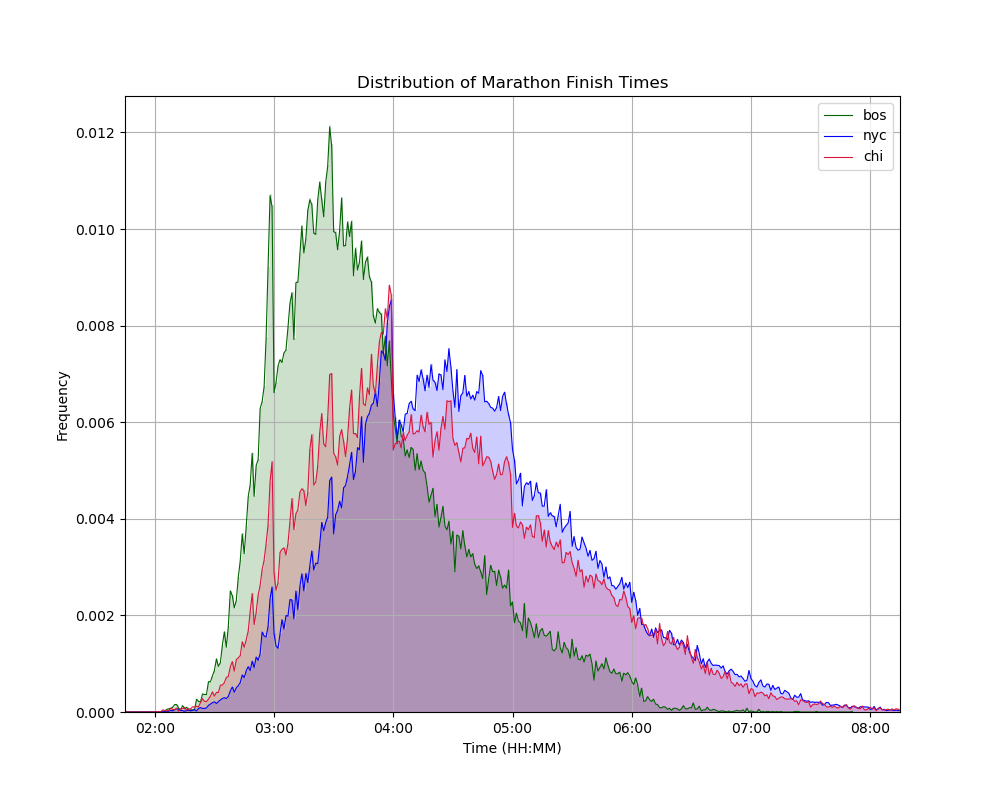
\includegraphics[width=4.2in]{../analysis/plots/plot_dist.png}
    \caption{Distribution of finish times for all finishers for each of the 3 marathons from 2021-2024}
    \label{fig:plotdist}
\end{figure*}

\subsection{Related Work} 
Marathon modeling using splits has been explored previously. Many methods have been explored for prediction of a finish time using splits. Machine learning such as k nearest neighbors  (Hammerling et al), Bayesian nonparametrics (Pradier et al). ...

In addition, other methods have been proposed to predict marathon times using various other predictor variables \cite{schmid:2012}. ...

Bayesian linear regression found many applications in many fields including \_. Collier \cite{collier:2017} explores using bayesian statistics for this problem. Hierarchical bayesian linear regression has been applied to \_.  ...

\section{Data} 
We focused our analysis on the three World Marathon Majors in the United States: the Boston Marathon, the New York City Marathon, and the Chicago Marathon. Each event hosts tens of thousands of runners every April, November, and October, respectively \cite{dredge:2025}. For the Boston Marathon, most runners qualify to compete by hitting notoriously difficult standards, while the remaining part of the 30,000-person field is made up of charity runner spots, which have no qualification standards. The New York City and Chicago Marathons, each with over 50,000 yearly runners, have lottery systems to select runners in addition to charity spots and time qualifiers. We scraped data for each marathon from the respective websites of each organization: Boston data was found on the Boston Athletic Association (BAA) website \cite{resultbos:2024}, New York City data on the New York Road Runners website \cite{resultnyc:2024}, and Chicago data on the Chicago Marathon website \cite{resultchi:2024}. 

Our 3 datasets (Boston, New York, Chicago) each contain the name, age, gender, and in-race splits (5K, 10K, 15K, 20K, HALF, 25K, 30K, 35K, 40K, and FINISH, all in seconds) for each finishing runner of the respective marathon from each race held since the COVID-19 pandemic (2021-2024). We decided to exclude runners who did not finish the race or do not have some or all intermediate splits recorded, as we only wanted to focus on runners that have all the information we want to use for prediction. We partitioned this data into 3 training sets (one for each marathon) of runners from years 2021-2023, and 3 corresponding test sets of runners from the year 2024. The values of the number of runners for each marathon in each year are shown in Table \ref{tab:counts}, and the distribution of the finish times for each marathon is shown in Fig. \ref{fig:plotdist}.

\begin{table}[!ht]
\centering
\begin{tabular}{c|ccc}
Year & Boston & New York & Chicago \\ \midrule
\csvreader[late after line = \\,]{../analysis/tables/race_info.csv}{}%
{\csvcoli & \csvcolii  & \csvcoliii & \csvcoliv}   \midrule 
Total & 90900 & 175780 & 167700 \\
 \end{tabular}
 \caption{Count of finishers for each marathon for each year}
 \label{tab:counts}
 \end{table}
 
\begin{figure*}[ht]
    \centering
    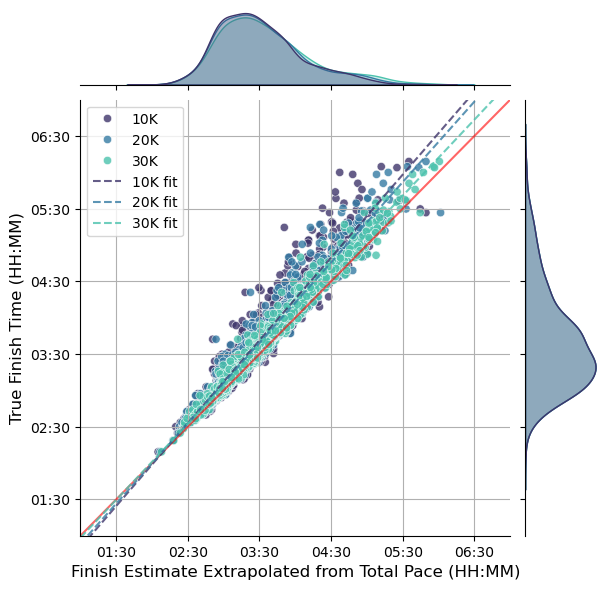
\includegraphics[width=4.2in]{../analysis/plots/bos_data_scatter.png}
    \caption{For three stages of the race (10K, 20K and  30K, in purple, blue, and cyan, respectively), the finish estimates extrapolated from the total pace so far (x-axis) are compared to the actual finish times (y-axis). The red line depicts the traditional estimate, while the other lines are the best fit lines for each of the three stages of the race.}
    \label{fig:scatter}
\end{figure*}

\subsection{Feature Modifications} 

By reformatting the data, we can get a more suitable set of features to perform our prediction task. For each stage of the race, we can compute the average pace (total distance covered so far, divided by total time, in m/s) of an individual runner up until that stage of the race. This feature, which we call the \emph{total\_pace}, forms the basis of the traditional method, which assumes that pace will be held constant for the rest of the race. In Fig. \ref{fig:scatter}, we directly compare true finish times with extrapolated \emph{total\_paces}, which represents the traditional method's finish time estimates. The red line represents the condition where the traditional method accurately predicts the finish time. For each of the different stages, most of the points lie above the traditional estimate line. We also plotted the best fit lines for each of the stages, and each one visually reflects a different relationship than the traditional method. In the next sections, we explore different possible relationships that could be used to predict finish times and evaluate the performance of each of the models.

%We also added features \emph{prop} and \emph{propleft}, which represent the proportion of distance covered and left to cover in the race for the runner, respectively (i.e., \emph{prop} is $(10,000 \text{m} / 42,195\text{m}) = 0.236$ when predicting for a runner at the 10K mark, whille \emph{propleft} is $1 - (25,000 \text{m} / 42,195\text{m}) = 0.407$ for a runner at the 25K mark).

Our other modification to the data was adding a \emph{curr\_pace} feature, which represents the pace of the most recently completed 5K for the runner. At the 5K mark, \emph{total\_pace} and \emph{curr\_pace} are the same, and for all other marks, the \emph{curr\_pace} value is computed from the splits. This is done by dividing 5000m by the time taken to run from the last stage to the current stage (\emph{curr\_pace} is also in m/s). This feature can show if there is a sudden recent change in a runner's pace, which can be helpful information for a more accurate final time prediction if a runner is starting to speed up or slow down dramatically.

\section{Methods}
\label{methods}

The traditional method of extrapolating the current pace (\textbf{extrap}) is used as a baseline. Here, the finish pace is assumed to be equal to \emph{total\_pace}. For our model, we wanted to represent the finish pace as a linear combination of features. Thus, for a collection of $N$ runners, we considered the following relationship.

\begin{equation}
f \sim  \mathcal{N}(XB, \sigma) %f \sim \matcal{N}(XB+\alpha, \sigma * p)
\label{eq:1}
\end{equation} %\[ finish \sim \mathcal{N}(XB + a, \sigma * propleft) \]

%$s \in \{1, 2, ..., 8\}$ is the stage of the race (1 = 5K, 2 = 10K, ..., 8 = 40K)
where $f \in \mathbb{R}^{N}$ is a vector for each runner's finish pace, $X \in \mathbb{R}^{N * D}$ is a feature matrix with $D$ features. The vector $B \in \mathbb{R}^{D}$ and value $\sigma$ are both parameters that need to be estimated. We explored the following candidate feature lists for $X$. \\

%We specified variance in the finish prediction ($\sigma * p$) to be proportional to $propleft$ because it represents the decrease in prediction uncertainty as the runner gets closer to the end of the race. We explored the following different feature lists for $X$.

\begin{itemize}
    \item \textbf{model1:} $[total\_pace ]$
    \item \textbf{model2:} $[total\_pace, curr\_pace ]$
    \item \textbf{model3:} $[total\_pace, curr\_pace, age, gender]$
\end{itemize}


We explored Bayesian linear regression models \cite{gelman:1995}, which incorporate Bayesian statistics by placing priors on the parameters of the linear regression model. By combining a likelihood function with a specified prior distribution, we form a posterior distribution of possible finish times for a given individual. We interpret the posterior both as a point estimate (using the median of the distribution) and a credible interval: a central region of the distribution we can use to quantify uncertainty. The Bayesian linear regression model is built using rstan, a library for creating and running Bayesian models \cite{stan:2024}.

We implement hierarchical Bayesian linear regression to better represent how the predictions vary based on how far into the race the runner is. Hierarchical regression is a compromise between two approaches: (1) pooling all the samples (corresponding to different stages) together to make parameter estimates, and (2) running separate models for each stage. We assume that there is a relationship between the distance into the race, but don't want to make assumptions about what this relationship is, so this model allows the parameters to share information. Thus, we can modify the equation above to get the following:

\begin{equation}
f_{s} \sim  \mathcal{N}(XB, \sigma_{s})
\label{eq:2}
\end{equation} 

where $s \in \{1, 2, ..., 8\}$ is the stage of the race (1 = 5K, 2 = 10K, ..., 8 = 40K). Here, $B \in \mathbb{R}^{s}$ is now a matrix and $\sigma \in \mathbb{R}^{s}$ is now a vector, both containing parameters to be estimated.

We can evaluate the performance of a Bayesian linear regression model by training on the training set (2021-2023) and predicting for runners in the test set (2024). We can compute the root mean squared error (RMSE) from the model for each runner and compare this to the RMSE of the extrapolation method on the same test set.

Increasing the number of features used to predict the finish times should reduce the RMSE and improve the accuracy of the predictions, as the model has more information to work with. We considered making predictions by directly incorporating all of the previous splits in the race to predict a future one, as this would contain the most prior information. However, we determined that this method has strong collinearity issues, as the previous splits of the runners are strongly correlated with each other. Furthermore, adding more features to the Bayesian model leads to significantly longer model runtimes, which makes the marginal gains in prediction accuracy negligible.  Especially with hierarchical regression, the number of parameter estimates grows rapidly with each additional feature. Thus, we opted to analyze in depth only the methods above and compare their performances to the baseline. 

For each marathon dataset, we subsampled our training set to randomly select 250 runners from 2021-2023 (giving us $250*8=2000$ individual samples), to speed up model training runtime while still having a reasonably sized data set to make inferences. We also sampled 4,000 runners (or 32,000 samples) for each test set.%The label extrap below represents the baseline extrapolation prediction.

\begin{table*}[!ht]
\centering
\begin{tabular}{c|c|cc|cc|cc}
 & extrap & \multicolumn{2}{c}{model1} & \multicolumn{2}{c}{model2} & \multicolumn{2}{c}{model3}  \\ \midrule 
Distance & RMSE & RMSE & \% Improve & RMSE & \% Improve & RMSE & \% Improve\\ \midrule
\csvreader[late after line = \\,]{../analysis/tables/bos_rmse.csv}{}%
{\csvcoli & \csvcolii  & \csvcoliii & \csvcolvi & \csvcoliv & \csvcolvii & \csvcolv & \csvcolviii}   \midrule
%& \csvcoliv & \csvcolv & \csvcolvi & \csvcolvii & \csvcolviii %& \csvcolix & \csvcolx
\csvreader[late after line = \\,]{../analysis/tables/bos_rmse2.csv}{}%
{\csvcoli & \csvcolii  & \csvcoliii & \csvcolvi & \csvcoliv & \csvcolvii & \csvcolv & \csvcolviii}   
\end{tabular}
 \caption{RMSE at different stages of the race for the traditional method and both Bayesian linear regression models}
 \label{tab:rmse}
 \end{table*}


\begin{figure*}[ht]
    \centering
    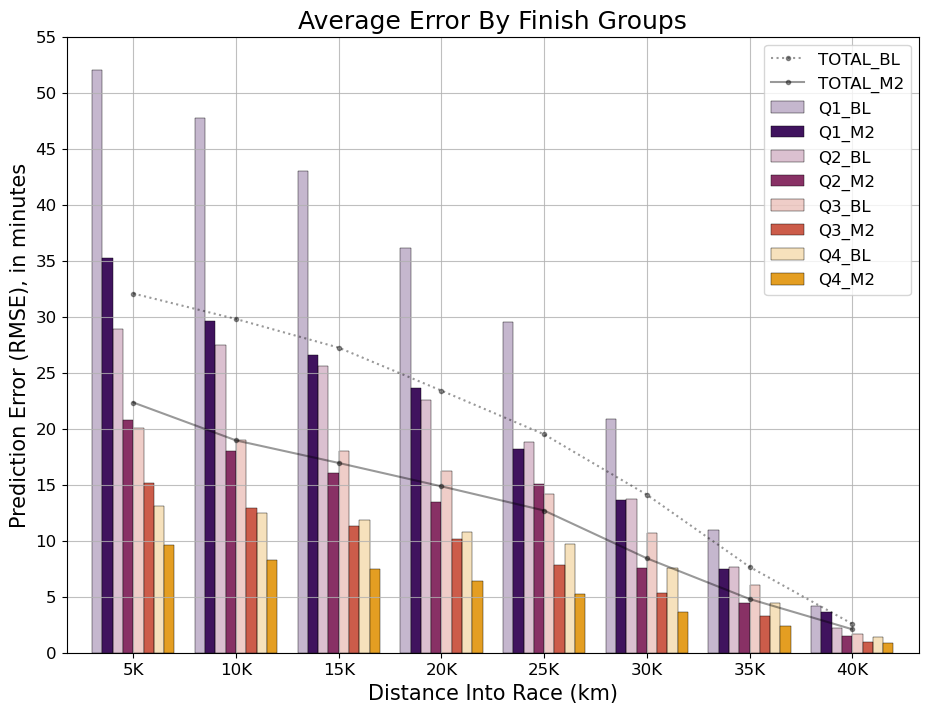
\includegraphics[width=4.2in]{../analysis/plots/bos_rmse_groups.png}
    \caption{RMSE at different stages of the race for the traditional method (lighter shades) and model2 (darker shades), broken down for different finishing groups, differentiated by color. The dotted and solid lines are the overall RMSE for traditional method and model2, respectively.}
     \label{fig:groups}
\end{figure*}

\section{Results}
\label{results}


The results, data, plots, and numbers mentioned in the following section are specifically from analysis using the Boston data set, for simplicity. Equivalent analyses were also completed from Chicago and New York, and discussion of the comparisons between these three marathons can be found in Section \ref{marathoncomparesection}. The decision to focus on model2 in Sections \ref{groupederrorsection} and \ref{credibleintervalsection} is explained in Section \ref{modelselectionsection}.

\subsection{Prediction Errors}
\label{predictionerrorsection}

As shown in Table \ref{tab:rmse}, all three of our models have similar test RMSE at most levels of the race. The models improve upon the traditional extrapolation method at all levels, and significantly outperform it in the beginning and middle stages of races, as shown by the improvement percentages. It is especially important to have better finish estimates earlier in the race, as there is the greatest amount of uncertainty at these stages. The gap in RMSE values decreases between the traditional model and our models in the latter stages of races (there is a less than one minute gap between our models and the traditional model at 40K compared to a 6-7 minute gap at 25K). This makes sense because the traditional model also benefits from decreased uncertainty at the latter stages of the race. This demonstrates that the overall pace alone is a strong estimator of the true overall finish pace when the race is almost done. % which makes sense 

Across all stages, model2 has slightly better performance than model1, although the gap is small compared to the gap between those models and the traditional one. Intuitively, this makes sense because having curr\_pace as an additional predictor gives enough information to get a slightly better estimate. Notably, model2 appears to have consistently better percentage improvement in the latter stages, while the model1 percentage improvement dips. Thus, there is a greater effect in having curr\_pace as the extra feature at those stages. The model3 RMSE is very similar to the model2 one, and we want to further analyze the effects of the extra features in model3 (age, gender) in Section \ref{modelselectionsection}.

Focusing on 15K, for example, we see that the model predictions, on average, are roughly 9-11 minutes closer to the actual finish time than the baseline predictions. When looking at our use case, this jump in performance is considerable, as users will benefit from having a much stronger prediction at a point in the race where there is high uncertainty. 

\subsection{Grouped Errors}
\label{groupederrorsection}

\begin{figure*}[ht]
    \centering
    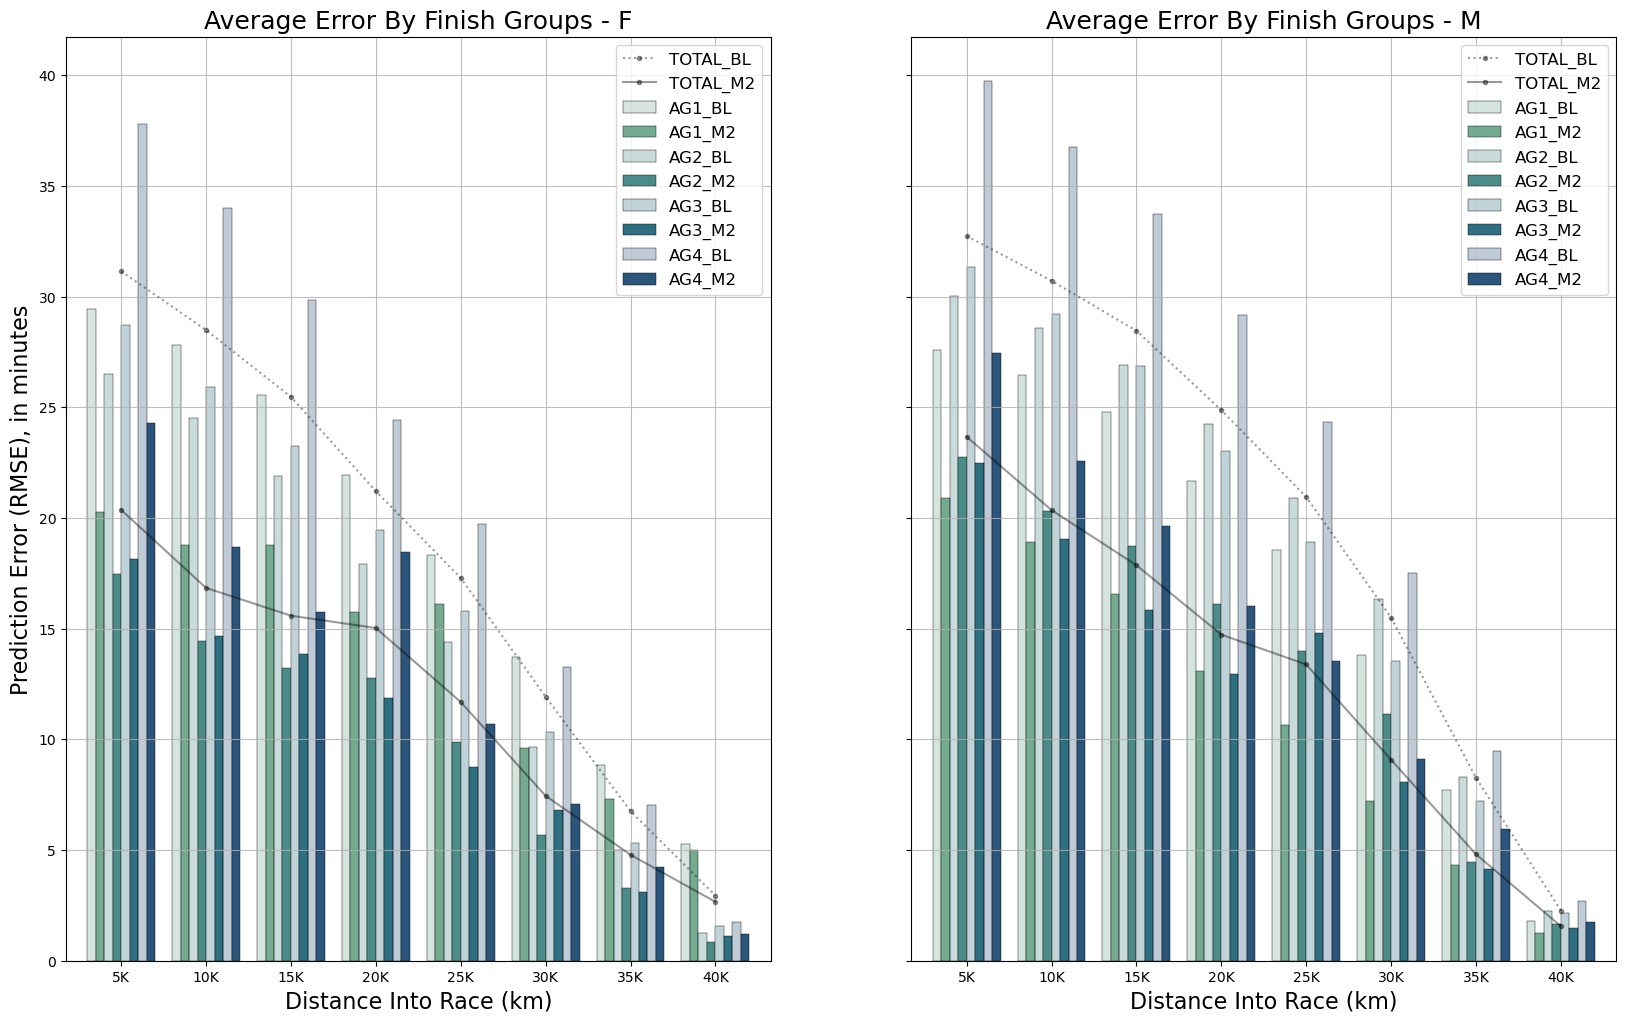
\includegraphics[width=6.2in]{../analysis/plots/bos_rmse_gender_age.png}
    \caption{RMSE at different stages of the race for the traditional method (lighter shades) and model2 (darker shades), broken down for different finishing groups, differentiated by color. The dotted and solid lines are the overall RMSE for traditional method and model2, respectively. The left plot is for female runners, while the right plot is for male runners.}
     \label{fig:breakdown}
\end{figure*}

We can examine this data further by looking at the breakdown of different groups within this test set. In Fig. \ref{fig:groups} the data is broken down into 4 equally partitioned finish groups (G4 being the fastest quarter of finishers, while G1 being the slowest quarter of finishers). We then show the RMSE values as bars for each group for both extrap and model2. This breakdown highlights how the prediction errors vary depending on how quickly you run. Generally, the slower runners have higher prediction errors, which makes sense because there is more variability in possible finishes with slower paces. 

%Interestingly, the model underperforms compared to the baseline method for the faster runners in the beginning stages of the race. G4 runners (the fastest quarter of runners) actually see the model underperforming until 20K, when the model starts outperforming the baseline for the rest of the race. G3 runners experience this until a switch at 15K, and even G2 runners experience this at 5K before a switch at 10K. G1 runners as a group consistently benefit from a model better than the baseline, which is very important given that these runners have the most uncertainty with their times.

It is important to note that this grouping arbitrarily examines the runners in quartiles, and a more fine-grained analysis, perhaps with more groups or better-defined groups, might reveal more about the model performance on specific cohorts of runners.

Another way to break down the data is categorizing runners by their age and gender, which is done in Fig. \ref{fig:breakdown}. Here, we grouped runners by both their gender and their "age groups" \footnote{Age group used in this context is distinct from how age groups are used in these marathons, which generally are in 5 year increments.}. Similar to how grouping worked above, AG4 refers to the oldest quarter of runners for a given gender, while AG1 refers to the youngest quarter of runners. This breakdown allows us to see prediction differences between age and gender. Overall, men have lower prediction errors than women. However, just as before, more can be learned with better-defined age groupings. %.....

\subsection{Credible Intervals}
\label{credibleintervalsection}

\begin{table*}[!ht]
\centering
\begin{tabular}{c|ccc|ccc|ccc}
 &  \multicolumn{3}{c}{50\%} & \multicolumn{3}{c}{80\%} & \multicolumn{3}{c}{95\%}  \\ \midrule 
Distance & model1 & model2 & model3 & model1 & model2 & model3 & model1 & model2 & model3 \\ \midrule
\csvreader[late after line = \\,]{../analysis/tables/bos_int_sizes.csv}{}%
{\csvcoli & \csvcolii  & \csvcoliii & \csvcoliv & \csvcolv & \csvcolvi & \csvcolvii & \csvcolviii & \csvcolix & \csvcolx}   \midrule     
\end{tabular}
 \caption{Average credible interval sizes at each stage of the race for model1 and model2}
      \label{tab:size}
 \end{table*}
The benefits of our models lie not only in the improved average accuracy of the finish time point estimates. For each individual, these models also provide a credible interval, used to quantify the uncertainty behind the estimate. When passing in a student's feature predictors at a given distance into one of the models, we can create an X\% credible interval $[t_1, t_2]$ such that the true finish time falls between $t_1$ and $t_2$ X\% of the time.

To validate the credible intervals generated from the models, we check how well they fit with our assumptions. Specifically, we examine the credible interval sizes. On average, we expect the credible interval sizes to decrease as one gets further into the race, which fits with our intuition that one should be more certain of the estimate as they get closer to finishing. We also expect that an X\% credible interval will be a larger size than a Y\% credible interval if $X < Y$. Table \ref{tab:size} shows that these generally hold true for three different credible intervals (50\%, 80\%, and 95\% intervals). Each average interval size decreases and converges towards 0 as the race progresses and gets closer to finishing, and 80\% intervals are narrower than 50\% intervals but larger than 95\% intervals. Notably, model2 consistently has smaller interval sizes than model1, showing that the extra information provides more certainty in the estimate.
 
We also want to see if, for a given X\% interval, approximately X\% of runners truly finish within that interval. This gives us an approximation to our true goal that an individual's finish time has an X\% chance of being within that predicted interval. Table \ref{tab:check} shows the proportions of intervals that contain the true value across different stages of the race for each model. The proportions are roughly around the expected proportions of 50\%, 80\%, and 95\%, but do not match up perfectly. 

 \begin{table*}[!ht]
\centering
\begin{tabular}{c|ccc|ccc|ccc}
 &  \multicolumn{3}{c}{50\%} & \multicolumn{3}{c}{80\%} & \multicolumn{3}{c}{95\%}  \\ \midrule 
Distance & model1 & model2 & model3 & model1 & model2 & model3 & model1 & model2 & model3 \\ \midrule
\csvreader[late after line = \\,]{../analysis/tables/bos_int_check.csv}{}%
{\csvcoli & \csvcolii  & \csvcoliii & \csvcoliv & \csvcolv & \csvcolvi & \csvcolvii & \csvcolviii & \csvcolix & \csvcolx}   \midrule
\end{tabular}
 \caption{Proportion of true finish times falling within credible intervals at each stage of the race for model1 and model2}
      \label{tab:check}
 \end{table*}

\subsection{Model Selection}
\label{modelselectionsection}

In selecting a model, we want to find a balance between choosing a model that has good performance and choosing one that is simple and has fewer parameters. Because all three models have similar RMSE values, we want to test if the slight differences between them are significant enough to warrant using a more complicated model over a simpler one. We tested this using the Kolmogorov–Smirnov test, a nonparametric test that determines if two samples come from the same distribution (H0: same distribution, H1: different distributions, p=0.05). Results of each comparison test are shown in the table below.

\begin{table}[!ht]
\centering
\begin{tabular}{c|ccc}
%Models & extrap, model1 & model1, model2 & model2, model3 \\ \midrule
1st Model & extrap & model1 & model2 \\ %\midrule
\textbf{2nd Model} & \textbf{model1} & \textbf{model2} & \textbf{model3} \\ \midrule
KS p-value & 0.0000 & 0.0000 & \underline{0.6033} \\
 \end{tabular}
 \caption{Kolmogorov–Smirnov test results comparing whether the model RMSE results come from the same distribution. Underlined are the not statistically significant results (p=0.05).}
 \label{tab:kstest}
 \end{table}
%ks test table

Thus, we cannot conclude that model3 and model2 are from different distributions. We verified this by also looking visually at the histograms of errors for all four models, and model2 and model3 looked the same overlayed (but slightly distinct from model1 and very distinct from extrap). Additionally, the model3 versions of Fig \ref{fig:groups} and Fig \ref{fig:breakdown} looked identical to the model 2 versions, showing that the result plot broken down by age and gender (model3's two additional features) is not significantly changed by incorporating them into the model. Combining all of this, we conclude that model3 is not significantly different enough from model2 to justify using it.

\subsection{Comparison Between Marathons}
\label{marathoncomparesection}

The Boston Marathon has lower prediction errors than the Chicago and New York Marathons. Looking back at Fig. \ref{fig:plotdist}, we can see that the Boston Marathon, as a whole, has a faster collection of runners than the other two marathons. This mostly comes down to the selection of runners, as Boston does not have a lottery that allows anyone to be able to run (only time qualifiers or charity runners can enter and run). This distribution difference affects how well models are able to predict. Additionally, races have different qualities (different courses, amount and placement of hills, typical race-day weather, levels of cheering support, etc.), which are all important factors. ...

[comparing RMSE values btw each marathon here]


\mycomment{
 \begin{table}[!ht]
\centering
\begin{tabular}{c|ccc}
 &  \multicolumn{3}{c}{RMSE model2} \\ \midrule 
Distance & Boston & New York & Chicago \\ \midrule
\csvreader[late after line = \\,]{../analysis/tables/marathons.csv}{}%
{\csvcoli & \csvcolii  & \csvcoliii & \csvcoliv i}   \midrule
\end{tabular}
 \caption{Proportion of true finish times falling within credible intervals at each stage of the race for model1 and model2}
      \label{tab:check}
 \end{table}
}
\section{Application}

We developed an application to display how the curr\_pace model can be used to make predictions for a marathon race in real time. The \emph{My Plot} tab of the app can be used to "simulate" a race; a user can select their marathon and sequentially enter in splits (in increments of 5K) and the app will dynamically compute and display finish time statistics. One output is a plot, displaying the predicted finish time probability distributions at different stages of the race. The centers of each curve represent the most probable finish times at that point of the race, and seeing multiple distributions together visually shows how the prediction changes over time. A narrower distribution represents more precise predictions and narrower credible intervals. The other output is a table showing the median finish time prediction as well as credible intervals (50\%, 80\%, and 95\%) for each stage of the race. This view of the data allows for a more detailed view of the actual values from the prediction. %The other tab (\emph{NUCR Plots}) shows the tables and plots of a few runners that ran the 2023 Boston Marathon, using the splits from their races.

\begin{figure}[ht]
    \centering
    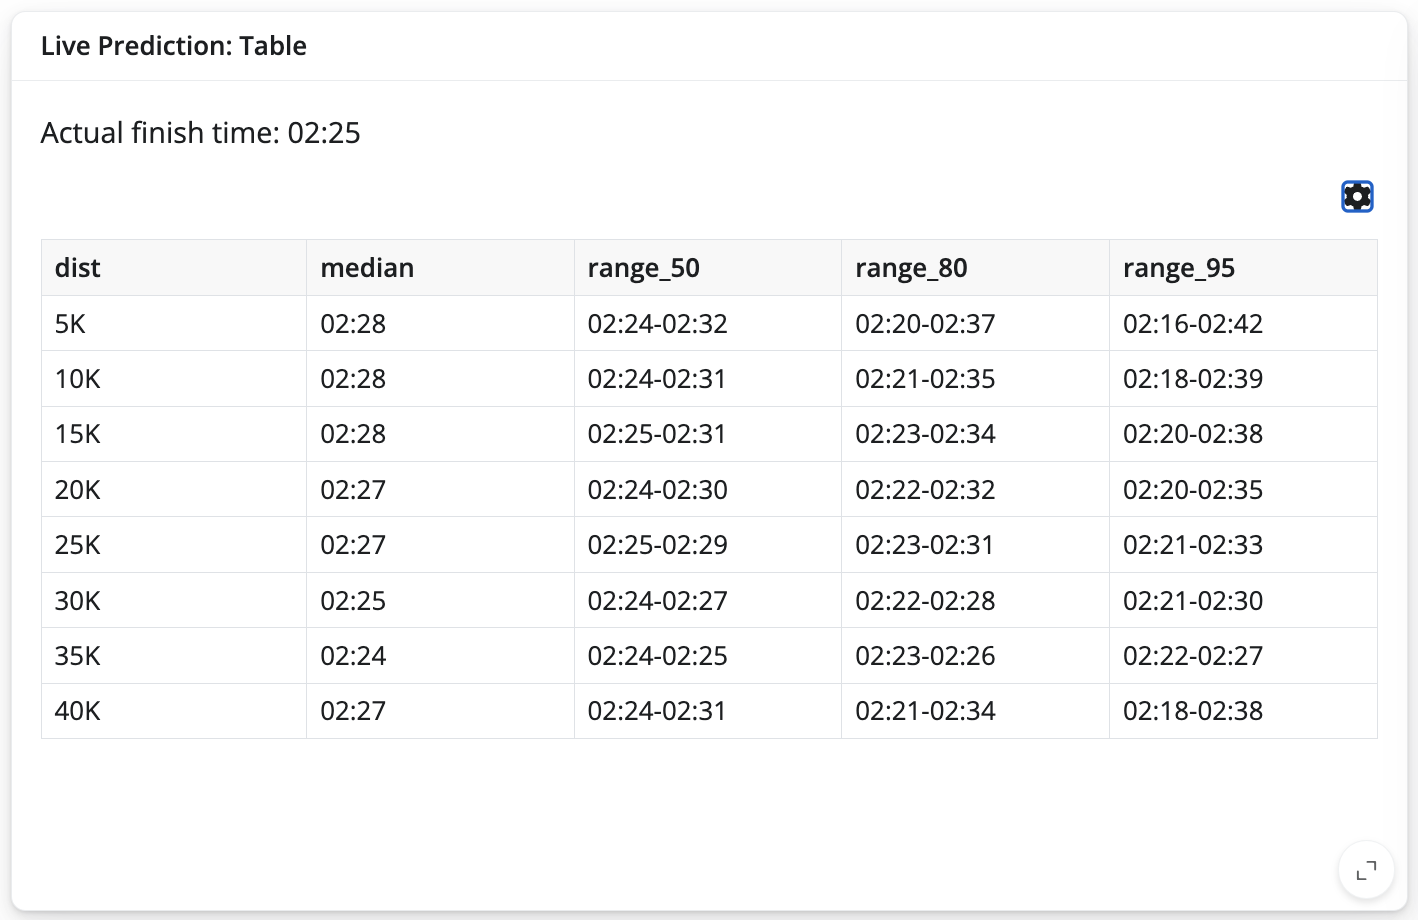
\includegraphics[width=3.2in]{app_screenshot1.png}
    \caption{Screenshot from the application. A table showing the median prediction as well as credible intervals (50\%, 80\%, and 95\%) at each stage of the race.}
\end{figure}

\begin{figure}[ht]
    \centering
    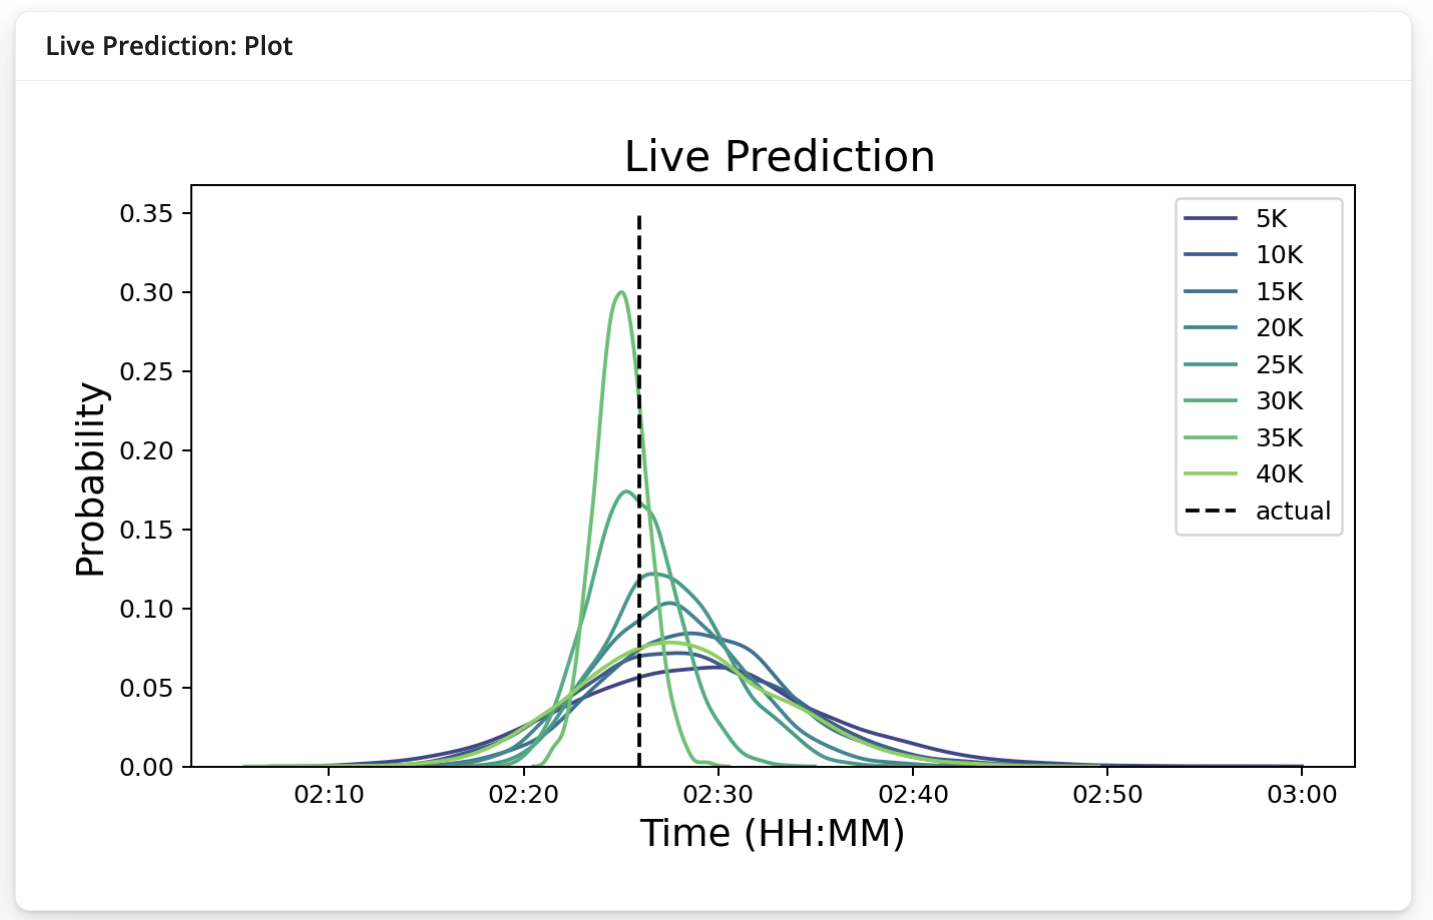
\includegraphics[width=3.2in]{app_screenshot2.png}
    \caption{Screenshots from the application.The probability distributions for finish times at each stage of the race shown in a plot.}
\end{figure}


The \emph{My Plot} tab can be a helpful tool to understand the distribution of possible finish times as the race is occurring. This can be used in a variety of contexts, whether for a coach informing a runner mid-race that they are on pace for their goal or not, a spectator trying to assess when their friend or family member will cross the finish line, or even the runner themselves after the race, analyzing how well they adhered to their race strategy. 

The app can be found at
\begin{center}
  \url{https://bonyejekwe.shinyapps.io/marathon_predictor/}
\end{center}


\section{Conclusion and Future Work}

Bayesian linear regression can be used to address the issues present in the traditional method of estimating marathon finish times. It benefits from significantly improved point estimates by taking into account the context of in-race splits, while simultaneously providing additional context around the estimate with credible intervals to provide a sense of uncertainty. What remains to be seen, however, is whether there are better predictor choices that could result in even better estimates from the models. While adding features significantly increases the time it takes to fit the Bayesian models, adding well-chosen features should help get better estimates. If we had access to other features, we could avoid the collinearity issues we discussed above with the method that incorporated all splits. In future work, we could better quantify the effects of feature selection on the overall RMSE for each model.

The application only implements our model of choice (model2) for simplicity. We decided that implementing multiple models could be overwhelming and unnecessary for the user, distracting from our goal to get fast and accurate information. However, by incorporating all of our models, there could be a visual comparison between them and could possibly reveal nuanced differences in the models if they give vastly different results for the same user. There is a subset of individuals in our test set where, for example, model1 had a better prediction than model2, so future work would involve examining that further and trying to find reasons why this affects some runners.

The model described in this paper and the resulting application were developed specifically to predict marathon finish times for these three marathon races. We ran the model 3 times for each dataset, and each resulted in different parameter estimates. Changing the dataset to the results of a different marathon will alter the predictions to make the model more applicable to that specific race. We would like to do further analysis on how specific marathons affect the parameter estimates in future work. We also noticed differences when training the models on different years. We know, for example, that weather can drastically change between years, which can affect how the runners pace and finish.

Finally, the prediction task can even be adapted towards different goals. For example, the model can be modified to predict when a runner will cross a certain point in the race (say, the 30km mark) instead of the finish, which can be helpful for a spectator stationed at that point wanting to know when a specific runner will pass by. 

All of the code used to create the analyses and develop the application can be found here: \url{https://github.com/bonyejekwe/Marathon_Predictor}

%.   %%%%%%%%%%%%%%%%%%%%%%%%%%%%%%%%%%

\begin{thebibliography}{9}
%Please refer to the journal's website for the corresponding reference style.

\bibitem{gelman:1995}
Gelman, A., Carlin, J. B., Stern, H. S., \& Rubin, D. B. (1995). \emph{Bayesian data analysis.} Chapman and Hall/CRC.

\bibitem{allen:2017}
Allen, E. J., Dechow, P. M., Pope, D. G., \& Wu, G. (2017). Reference-dependent preferences: Evidence from marathon runners. \emph{Management Science, 63}(6), 1657-1672.

\bibitem{kwong:2019}
Kwong, H. S., \& Nadarajah, S. (2019). Modelling dynamics of marathons–A mixture model approach. \emph{Physica A: Statistical Mechanics and its Applications}, 534, 120798.

\bibitem{resultbos:2024}
\emph{Results: Boston Athletic Association.} Results | Boston Athletic Association. (2024). \url{https://www.baa.org/races/boston-marathon/results}

\bibitem{resultnyc:2024}
\emph{NY Race Results}  \url{https://www.nyrr.org/tcsnycmarathon/results/race-results}

\bibitem{resultchi:2024}
\emph{CHI Race Results} \url{https://www.chicagomarathon.com/runners/race-results/}

\bibitem{perktold:2024}
Perktold, J., Seabold, S., \& Taylor, J. (2024). \emph{Quantile regression}. Quantile regression 
- statsmodels 0.15.0 (+431). \url{https://www.statsmodels.org/dev/examples/notebooks/generated/quantile_regression.html}

\bibitem{coder:2024}
\emph{GLM: Linear regression}. GLM: Linear regression - PyMC 5.16.2 documentation. (2024). \url{https://www.pymc.io/projects/docs/en/stable/learn/core_notebooks/GLM_linear.html} 

\bibitem{dredge:2025}
\emph{How to Get Into the World Marathon Majors}.  (2025). \url{https://therunningchannel.com/how-to-get-into-the-world-marathon-majors/} 

\bibitem{stan:2024}
Stan Development Team \emph{RStan: the R interface to Stan} \url{https://mc-stan.org/}

\bibitem{collier:2017}
Andrew Collier. \emph{Bayesian Marathon Predictions} \url{https://datawookie.dev/blog/2017/02/bayesian-marathon-predictions}

\bibitem{pradier:2016}
F. Pradier M, J. R. Ruiz F, Perez-Cruz F (2016) Prior Design for Dependent Dirichlet Processes: An Application to Marathon Modeling. PLOS ONE 11(1): e0147402. https://doi.org/10.1371/journal.pone.0147402

\bibitem{hammerling:2014}
Hammerling D, Cefalu M, Cisewski J, Dominici F, Parmigiani G, et al. (2014) Completing the Results of the 2013 Boston Marathon. PLOS ONE 9(4): e93800. https://doi.org/10.1371/journal.pone.0093800

\bibitem{berndsen:2019}
Jakim Berndsen, Barry Smyth, and Aonghus Lawlor. 2019. Pace my race: recommendations for marathon running. In Proceedings of the 13th ACM Conference on Recommender Systems (RecSys '19). Association for Computing Machinery, New York, NY, USA, 246–250. https://doi.org/10.1145/3298689.3346991

\bibitem{schmid:2012}
Schmid W, Knechtle B, Knechtle P, Barandun U, Rst C A, et al. Predictor Variables for Marathon Race Time in Recreational Female Runners.Asian J Sports Med.2012;3(2):34704.https://doi.org/10.5812/asjsm.34704.

\bibitem{munoz:2024}
Muñoz-Pérez, I., Castañeda-Babarro, A., Santisteban, A. et al. Predictive performance models in marathon based on half-marathon, age group and pacing behavior. Sport Sci Health 20, 797–810 (2024). https://doi.org/10.1007/s11332-023-01159-4

\bibitem{stan:2025}
Stan User Guide: Regression Models. \url{https://mc-stan.org/docs/stan-users-guide/regression.html#hierarchical-regression}

\end{thebibliography}

%\newpage \newpage

\section{TODO (Updated 8/5/25):}
\begin{itemize}
	\item 1) Related work section
	\item 2) Add to comparison btw marathons section
	\item 3) Fix citations throughout paper
	\item 4) Clean up Methods section (formula notation)
	\item 5) Clean up Model Selection section (statistical test)
	\item 6) scrape age/gender data for Chicago
	\item 7) maybe add section discussing fitted parameter values
\end{itemize}

\appendix
\section{Below: Unorganized collection of plots / tables currently}

 \begin{table}[!ht]
\centering
\begin{tabular}{c|c|cc|cc|cc}
 & extrap & \multicolumn{2}{c}{model1} & \multicolumn{2}{c}{model2} & \multicolumn{2}{c}{model3}  \\ \midrule 
Distance & RMSE & RMSE & \% Improve & RMSE & \% Improve & RMSE & \% Improve\\ \midrule
\csvreader[late after line = \\,]{../analysis/tables/nyc_rmse.csv}{}%
{\csvcoli & \csvcolii  & \csvcoliii & \csvcolvi & \csvcoliv & \csvcolvii & \csvcolv & \csvcolviii}   \midrule
%& \csvcoliv & \csvcolv & \csvcolvi & \csvcolvii & \csvcolviii %& \csvcolix & \csvcolx
\csvreader[late after line = \\,]{../analysis/tables/nyc_rmse2.csv}{}%
{\csvcoli & \csvcolii  & \csvcoliii & \csvcolvi & \csvcoliv & \csvcolvii & \csvcolv & \csvcolviii}   
\end{tabular}
 \caption{ NEW YORK RMSE TABLE}
 \label{tab:rmse2}
 \end{table}
 
  \begin{table}[!ht]
\centering
\begin{tabular}{c|c|ccc|ccc}
&  \multicolumn{4}{c}{RMSE}  &  \multicolumn{3}{c}{\% Improvement from extrap}  \\ \midrule
Distance & extrap & model1 & model2 & model3 & model1 & model2 & model3   \\ \midrule 
\csvreader[late after line = \\,]{../analysis/tables/bos_rmse.csv}{}%
{\csvcoli & \csvcolii  & \csvcoliii & \csvcoliv & \csvcolv & \csvcolvi & \csvcolvii & \csvcolviii}   \midrule 
\csvreader[late after line = \\,]{../analysis/tables/bos_rmse2.csv}{}%
{\csvcoli & \csvcolii  & \csvcoliii & \csvcolvi & \csvcoliv & \csvcolvii & \csvcolv & \csvcolviii}   
\end{tabular}
 \caption{ALTERNATIVE FORMAT TO MAIN RMSE TABLES ABOVE}
 \end{table}


\begin{figure*}[ht]
    \centering
    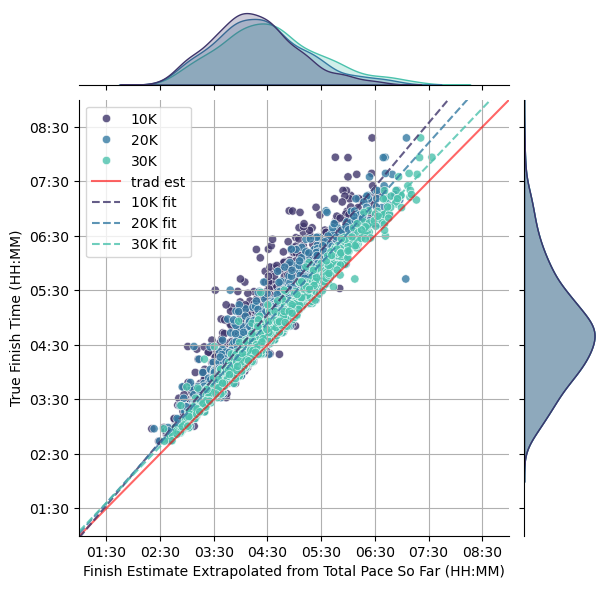
\includegraphics[width=2.7in]{../analysis/plots/nyc_data_scatter.png}
    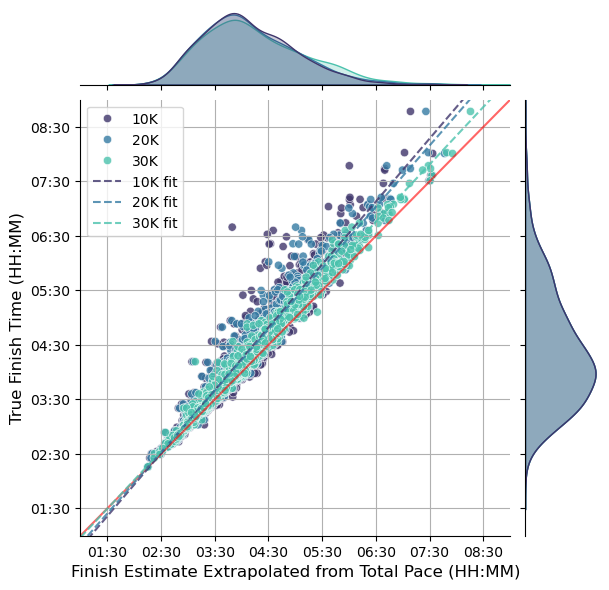
\includegraphics[width=2.7in]{../analysis/plots/chi_data_scatter.png}
    \caption{SCATTERPLOT (NEW YORK LEFT, CHICAGO RIGHT)}
\end{figure*}

\begin{figure*}[ht]
    \centering
    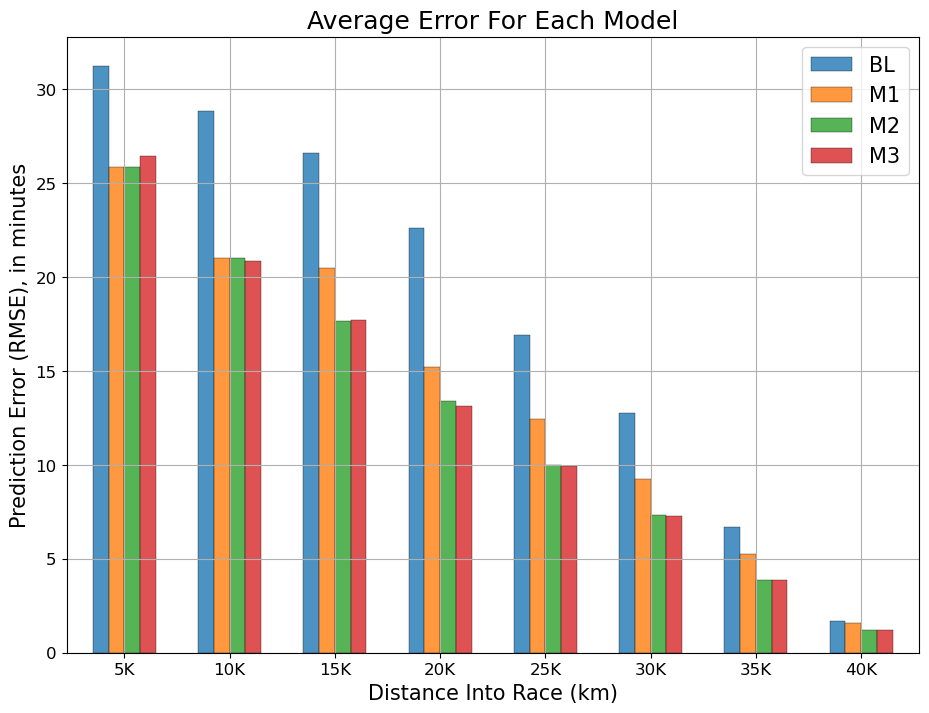
\includegraphics[width=2.7in]{../analysis/plots/nyc_rmse_bar.png}
    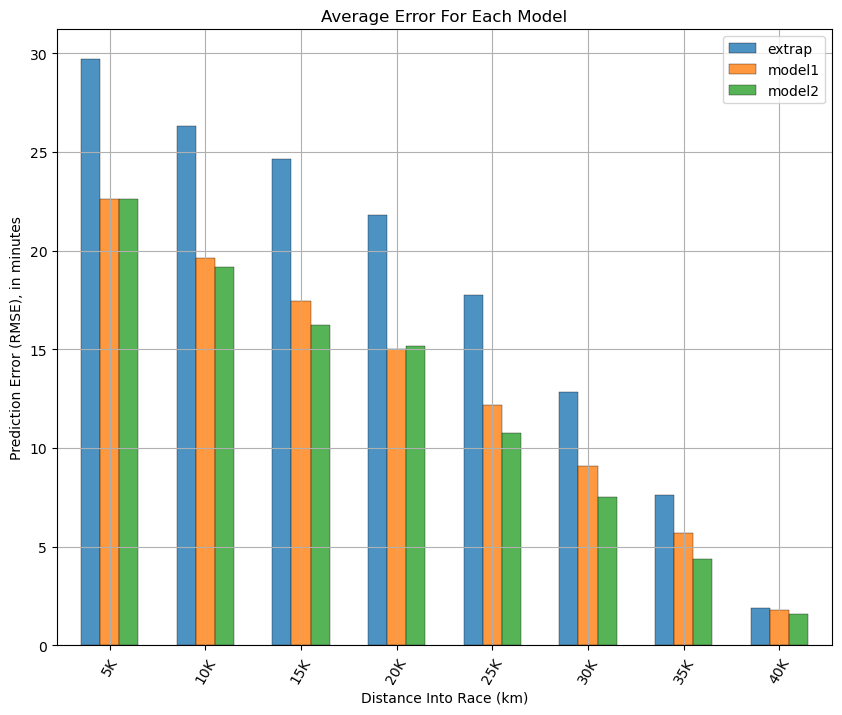
\includegraphics[width=2.7in]{../analysis/plots/chi_rmse_bar.png}
    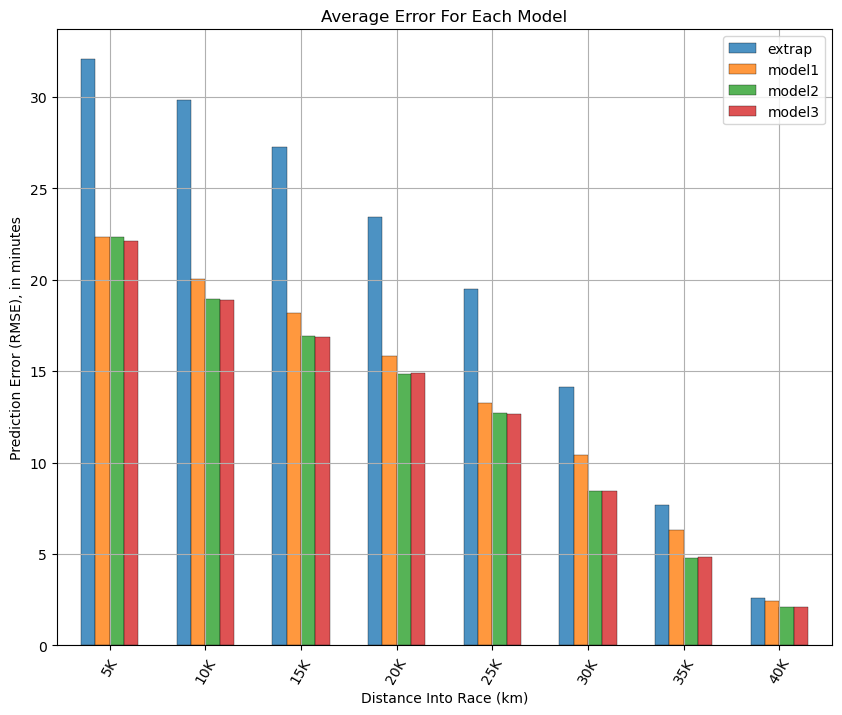
\includegraphics[width=2.7in]{../analysis/plots/bos_rmse_bar.png}
    \caption{RMSE AS BAR PLOT INSTEAD OF TABLE (NEW YORK LEFT, CHICAGO RIGHT, BOSTON BOTTOM)}
\end{figure*}

\begin{figure*}[ht]
    \centering
    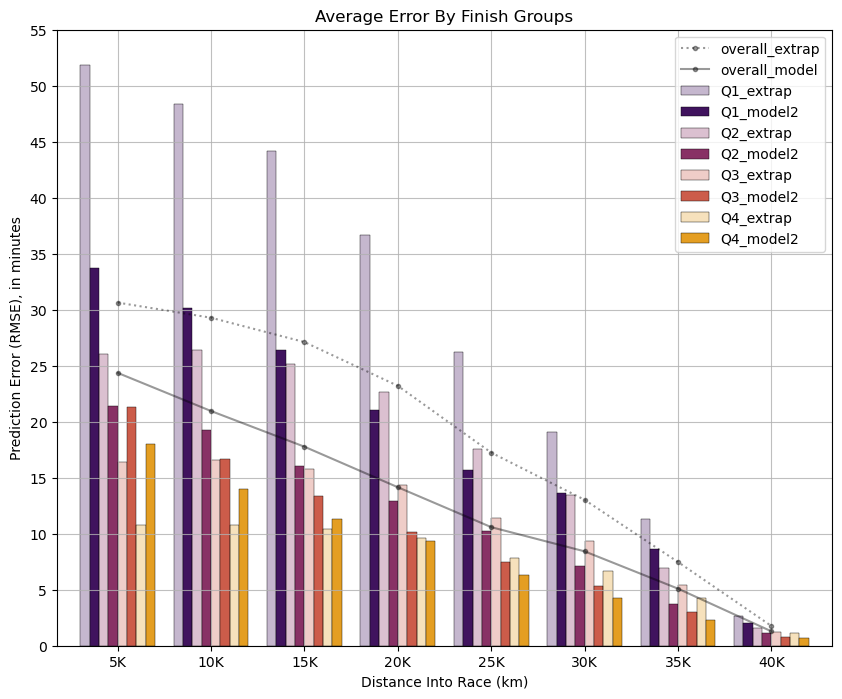
\includegraphics[width=2.7in]{../analysis/plots/nyc_rmse_groups.png}
    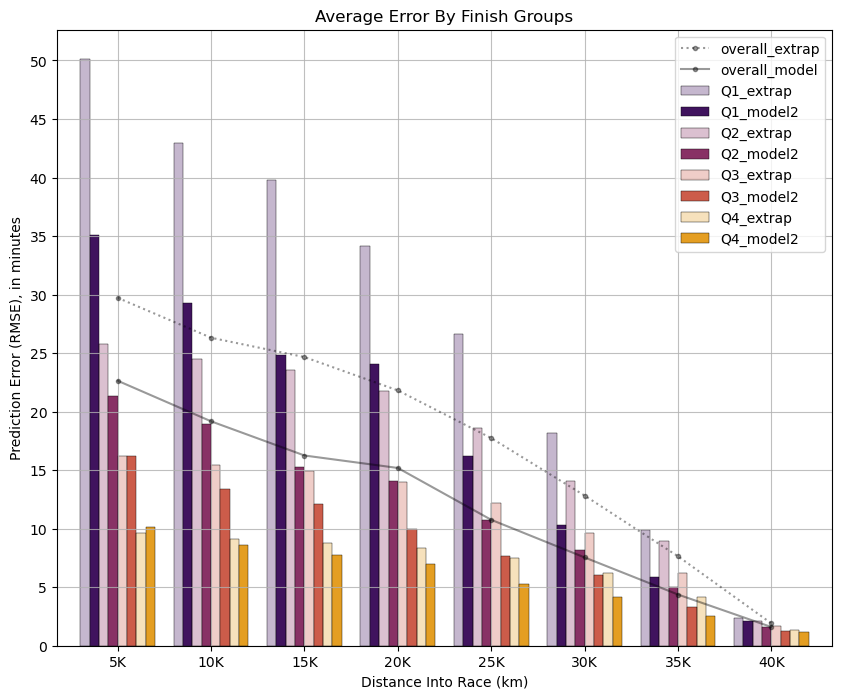
\includegraphics[width=2.7in]{../analysis/plots/chi_rmse_groups.png}
    \caption{RMSE GROUPED. (NEW YORK LEFT, CHICAGO RIGHT)}
\end{figure*}

\begin{figure*}[ht]
    \centering
    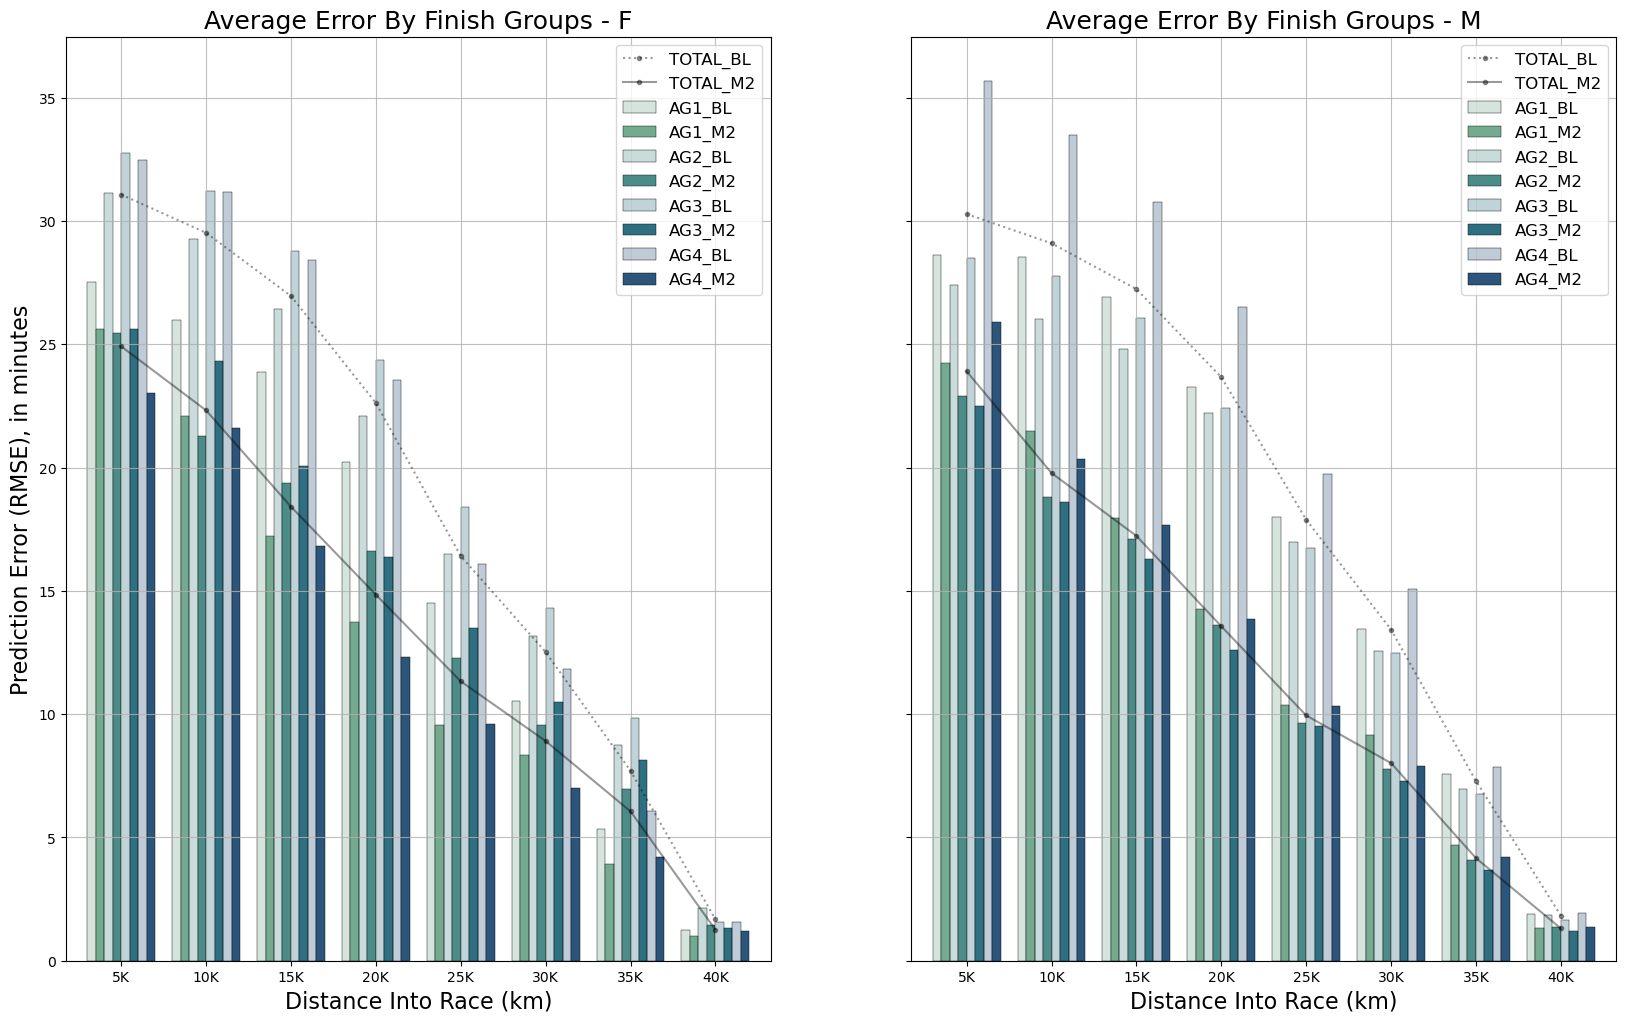
\includegraphics[width=6.2in]{../analysis/plots/nyc_rmse_gender_age.png}
    \caption{RMSE  GROUPED AGE/GENDER (NEW YORK)}
\end{figure*}

\begin{figure*}[ht]
    \centering
    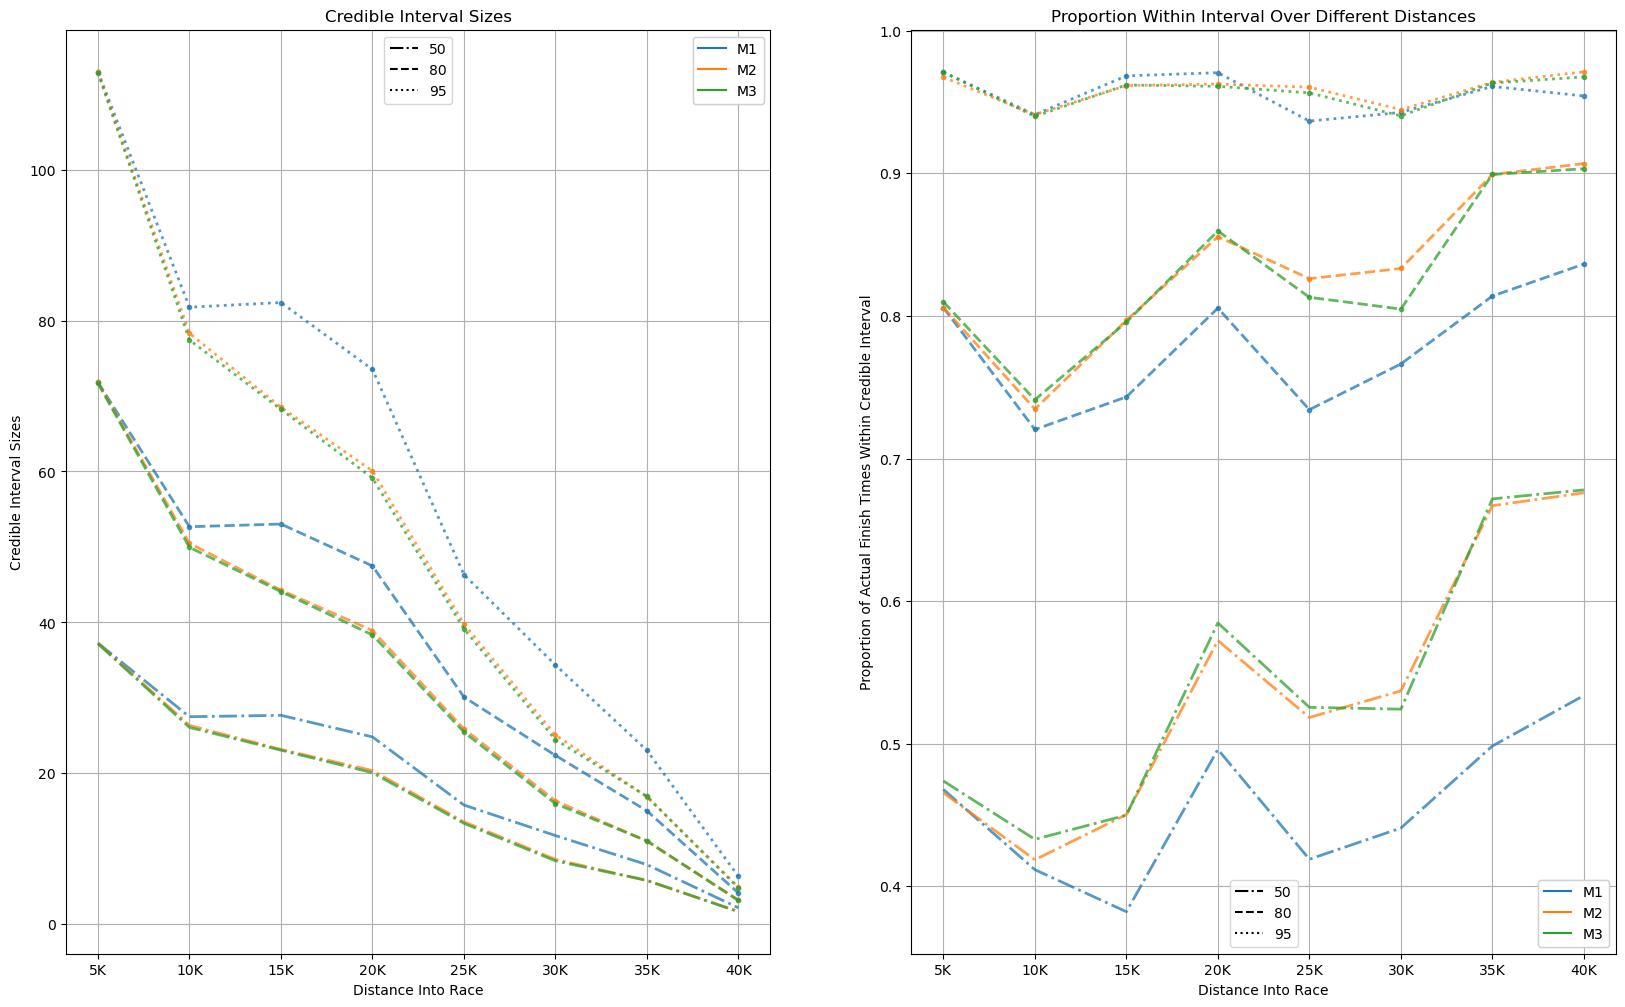
\includegraphics[width=2.7in]{../analysis/plots/nyc_intervals.png}
    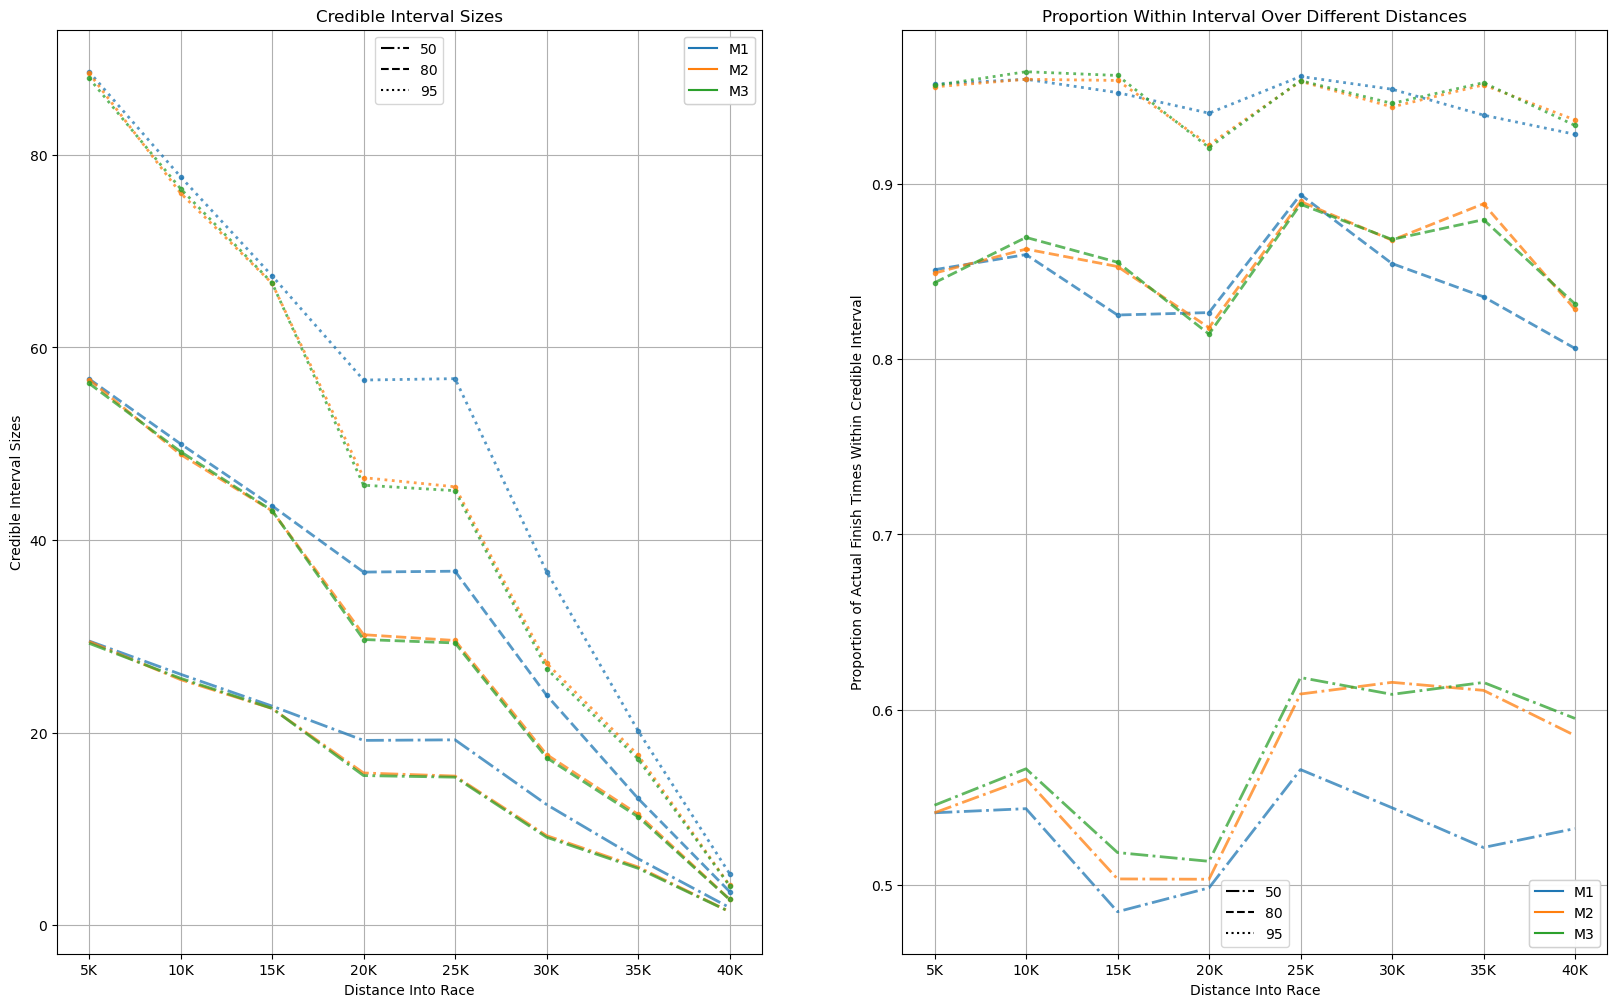
\includegraphics[width=2.7in]{../analysis/plots/chi_intervals.png}
     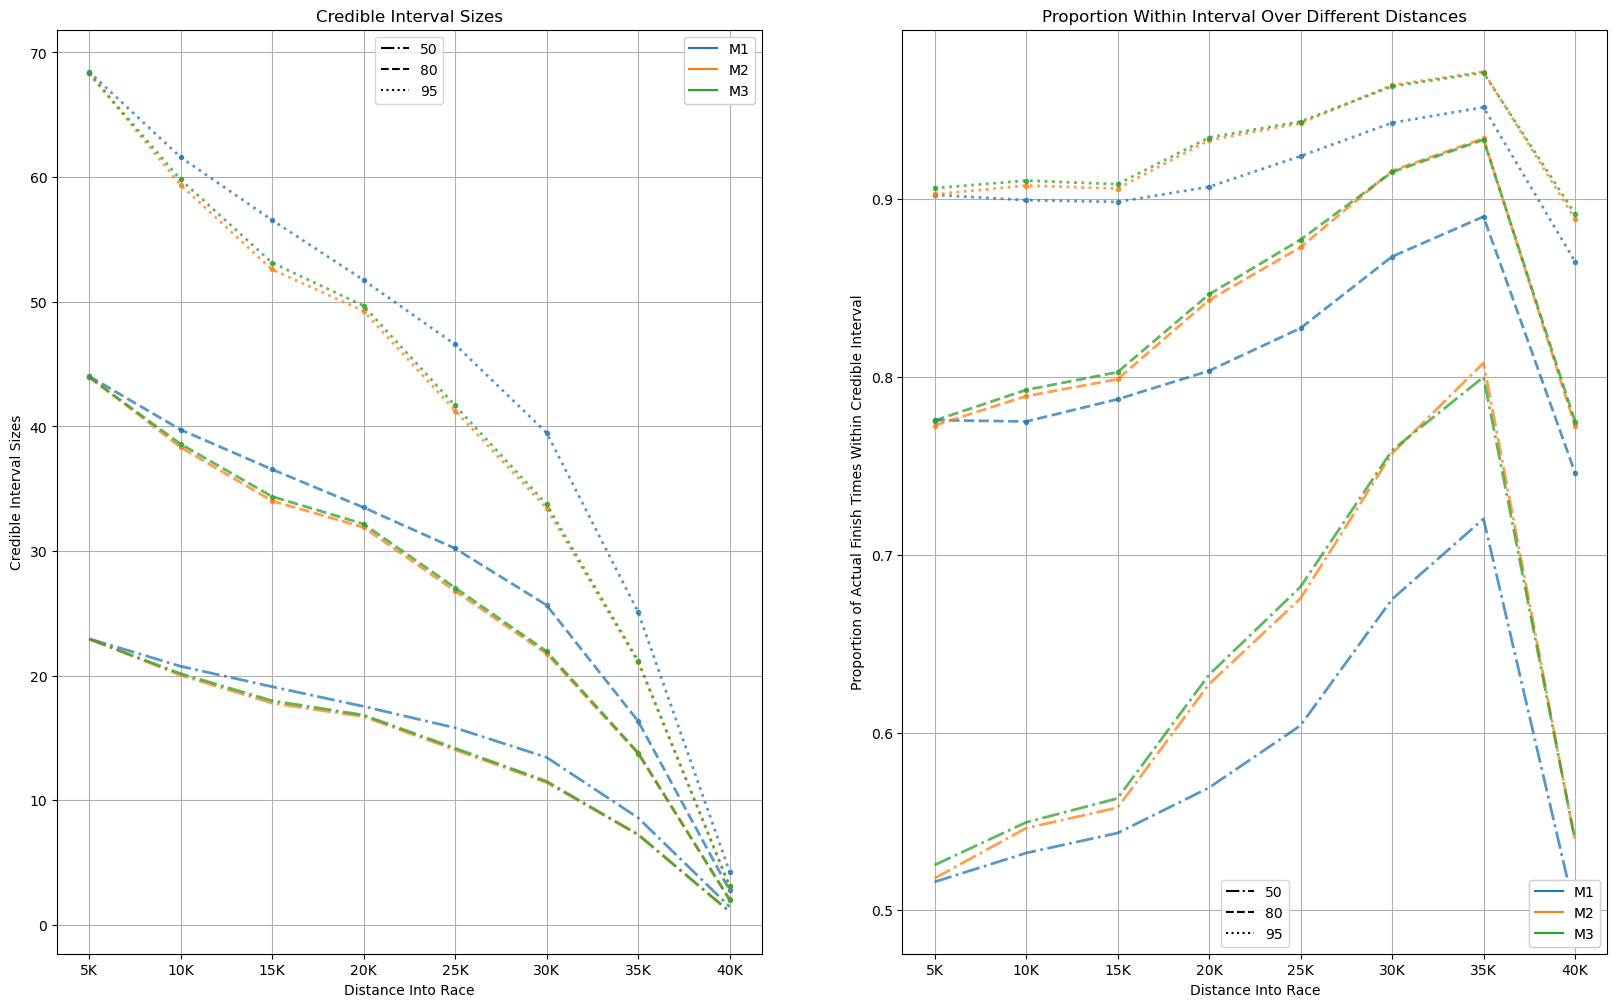
\includegraphics[width=2.7in]{../analysis/plots/bos_intervals.png}
    \caption{CREDIBLE INTERVAL SIZES AND PROPORTION WITHIN INTERVAL (NEW YORK LEFT, CHICAGO RIGHT, BOSTON BOTTOM)}
\end{figure*}
%}

\end{document}
